\documentclass{article}

\usepackage{hyperref,graphicx,tikz}
\usetikzlibrary{decorations.pathmorphing}

\begin{document}

\newcommand{\todo}[1]{\vspace{.5cm} TODO: #1 \vspace{.5cm}}

\section{Project description}

You will create a multithread application to simulate life of autonomous worms.
All the worms will be placed within the same environment and will interact
with each other. The goal is to simulate an ecosystem with diverse types
of individuals living inside.

\begin{center}
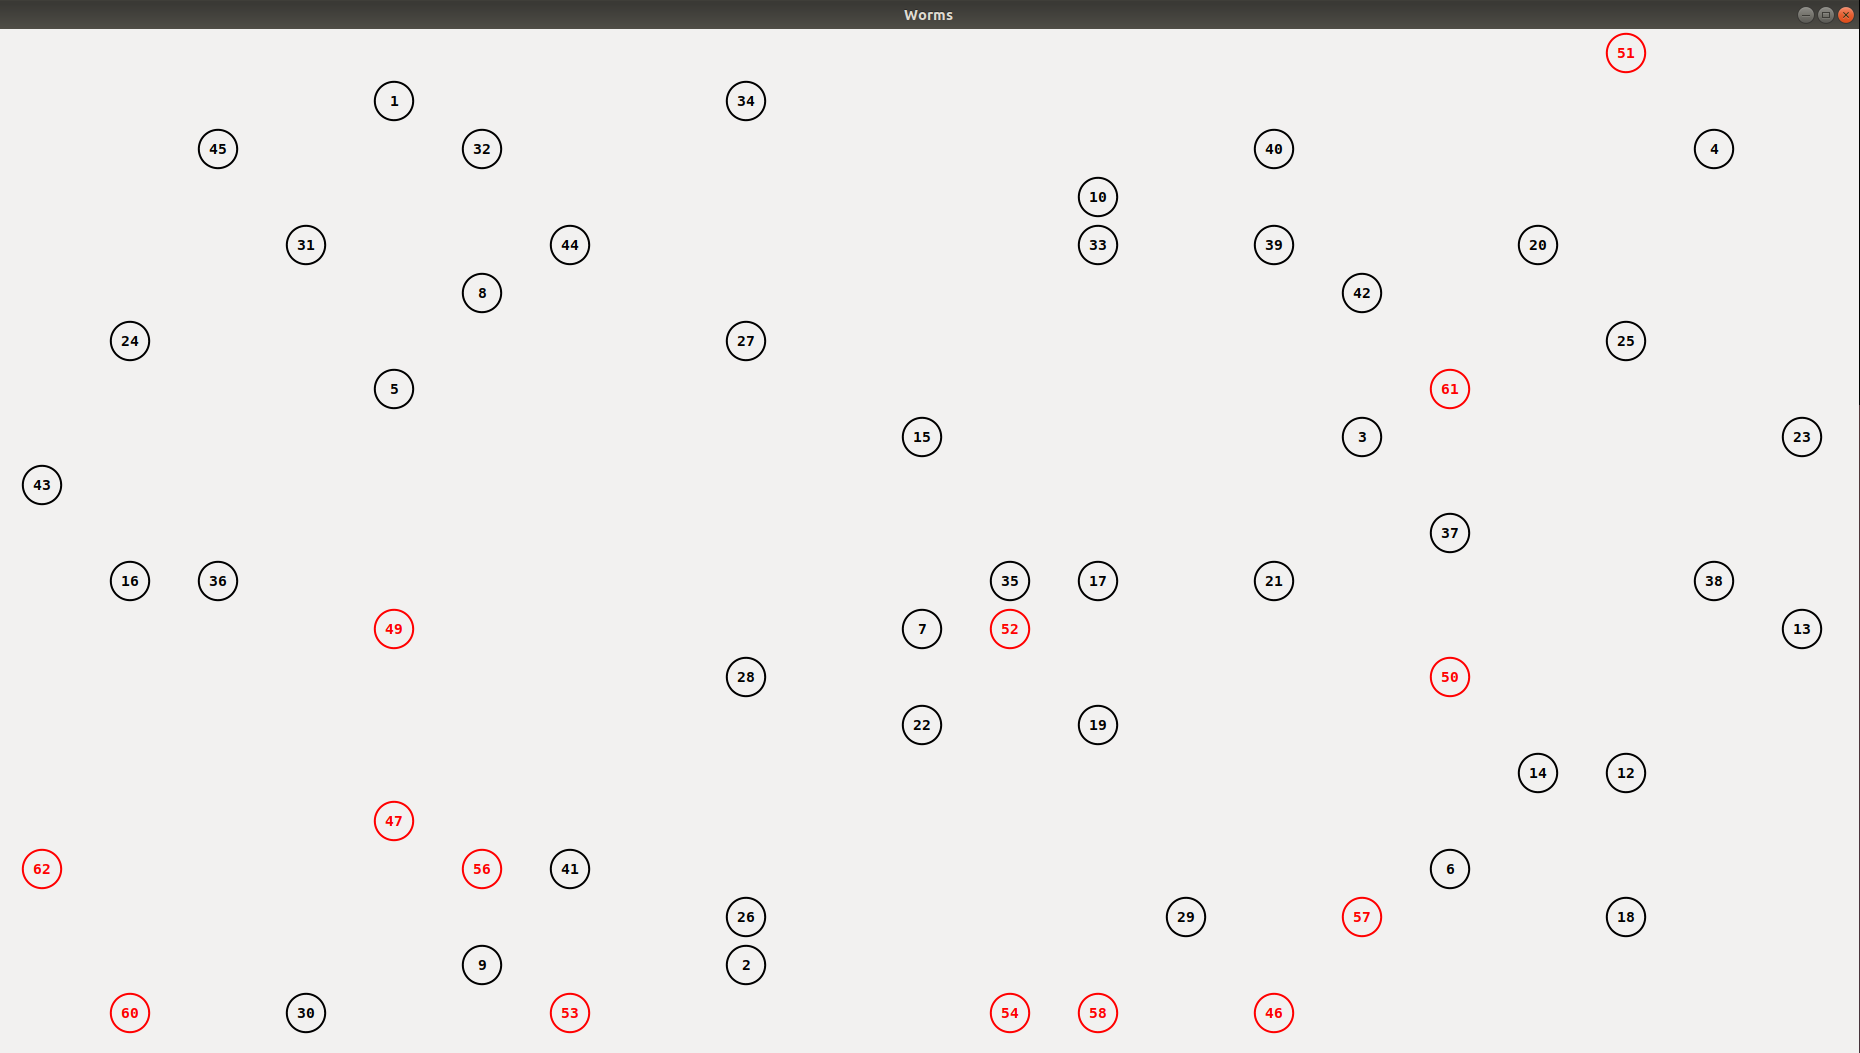
\includegraphics[width=12cm]{wormsApp}
\end{center}

All worms will live on a ractangular ground, where hitting an edge results
in appearing on the other side. Similar to the
\href{https://elgoog.im/snake/}{\textit{Snake}} game available on old Nokia
phones. In other words, the environment is a torus projection on a 2D
screen.

\begin{center}
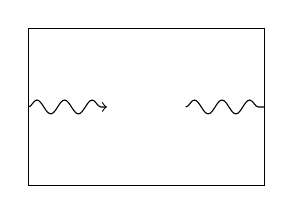
\begin{tikzpicture}
  \draw (0,0) rectangle (3,2);
  \draw[decorate, decoration=snake] (2,1) -- (3,1);
  \draw[->, decorate, decoration=snake] (0,1) -- (1,1);
\end{tikzpicture}
\end{center}

The design of the core functionality with two types of worms has been prepared,
together with an implementation with a few missing functionalities. You will
need to implement them to make the application run and to satisfy predefined
test cases and later you will prepare your own design for the extensions
of the application.

\subsection{Worms movements}

Board is a square grid where all the worms are placed. Each worm is entirely
within one of the fields (i.e. $(1,1)$) and has its own identifier which
is visible in debug mode. A worm may choose any adjacent field to move,
but if on the desired field is already a worm placed then it will be eaten
by the one taking the step. It means that when two worms are in adjacent
fields and both deside to eat each other then the winner is the one whose
thread will execute this first.

\subsection{Interactions between worms}

There will be two types of worms (you will make additional types in
\textit{extended functionality}):
\begin{itemize}
  \item \textit{Lazy Worm (black)}
  \item \textit{Hunter Worm (red)}
\end{itemize}

\subsubsection{\textit{Lazy Worm (black)}}

This worm randomly travels around. Complete random movements don't look
realistic, so it has some direction he's currently moving
(i.e. left which means going directly to the left border of the application window)
and with probability 75\% it keeps that direction. It turns left (relatively
to the current direction) in 12.5\% times and right (relative) with 12.5\% chance.

\subsubsection{\textit{Hunter Worm (red)}}

This worm choses a goal on the board and moves towards it. Of course possible
targets are constantly moving around, so the goal coordinates need to be updated.
Before each step he is locating the desired item on the board, updates the
coordinates he's heading to and then performs a move towards it. If the goal
(i.e. other worm) disappeared (was eaten) then a new goal is chosen which is
closest in distance. When nothing is left on the board he choses to reach
a random field on the board.

\section{Technical specification}

\subsection{Sources}

Project package contains a directory with source codes, makefile and tests.
It should follow best practices of a multithread application and a style
guidelines.

Source files with main logic are available in \texttt{sources/}, all tests
are within \texttt{tests/}. Your first modifications will need to be made
in \texttt{sources/worm.cpp} and \texttt{sources/board.cpp}.

\subsection{Debugging}

Tha application has debug mode which draws all the worm ids on the board
instead of plain circles. You may turn it on by changing the very last
parameter of call function \texttt{createAndRun} to \texttt{true} within
\texttt{main.cpp} file. You may also want to modify other parameters
to change the size of the board (cureently it is 20x20 fields).

\section{Basic functionality}

List of files that need to be modified for the whole application to run:
\begin{itemize}
  \item \texttt{sources/worm.cpp}
  \item \texttt{sources/board.cpp}
\end{itemize}

List of functions to implement:
\begin{itemize}
  \item \texttt{move} function that based on \texttt{currDir\_} which is the
    current worm direction (\texttt{LEFT, RIGHT, UP} or \texttt{DOWN}) performs
    one step towards it by modifying appropriate class variables,
  \item \texttt{addWorm} function that should add new worm into the internal
    board at given coordinates, give it an appropriate id
    (see \texttt{nextId\_}) and run the thread (\textit{hint:}
    \href{https://en.cppreference.com/w/cpp/container/unordered\_map/emplace}{\texttt{emplace}}
    method will be useful),
  \item find appropriate function and implement joining the threads.
\end{itemize}

List of basic functionality needed to add:
\begin{itemize}
  \item \textbf{synchronization} -- currently no synchronization is implemented,
    so threads (worms) may create race conditions on the board (they kill each
    other and update their location),
  \item \textbf{error handling / exceptions} -- currently all the errors are printed to
    the standard output using \texttt{std::cout} and some are
    not handled at all (like giving incorrect board size which should definitely
    greater than $0$).
\end{itemize}

\section{Extended functionality}

When finished with basic functionality you will need to extend your application
to become interesting to watch. It will engage you to shape your code
in a way that fits the core design, but extension's design will be entirely
up to you.

Extensions (detailed explanation in a separate section of this document):
\begin{itemize}
  \item Implement bonuses (small items like cherries) that appear randomly
    on the board,
  \item Save function that allows to dump current state into a file (and load
    it during the next run),
  \item (big) Implement behaviour schema for a worm, basically artificial
    intelligence,
\end{itemize}


\subsection{Bonuses}

Once in a while on the board may appear additional item -- bonus -- which
will be desired by the worms. It doesn't need to actually give any points
or anything, but worm's logic may prioritize to collect it and make the whole
,,show'' more interesting.

\textit{Notice:} This task may require to get familiar with \texttt{graphics.*}
and \textit{gtkmm} library for drawing. It would be sufficient to draw circles
of a different color (i.e. blue) to make it distinguishable from other objects.

\subsection{File dump}

The whole board may be dumped into a file (together with worms locations)
and retrieved during next run. Since it is not possible to dump exact threads
and their contexts it is enough to create a new worm of a correct type
within a place of a dumped one.

\subsection{Artificial intelligence}

Provided worms have very limited ,,thinking'' -- it would be interesting to see
actual ,,smart'' worms who use some clever ideas of your own to make this
battle spectacular.


\vspace{1cm}
\textbf{Good luck!}


\end{document}
